\documentclass[seminarskirad]{fer}

\usepackage{blindtext}
\usepackage{hyperref}
\usepackage{listingsutf8}

\input{Quickstart Examples/lstlistings.txt}
\lstset{style=ckod}

%--- PODACI O RADU / THESIS INFORMATION ----------------------------------------

% Naslov na engleskom jeziku / Title in English
\title{ESP-NOW protocol}

% Naslov na hrvatskom jeziku / Title in Croatian
\naslov{ESP-NOW protokol}

% Autor / Author
\author{Fran Fodor}

% Mentor 
\mentor{Doc. dr. sc. Leonardo Jelenković}

% Datum rada na engleskom jeziku / Date in English
\date{June, 2025}

% Datum rada na hrvatskom jeziku / Date in Croatian
\datum{lipanj, 2025.}

%-------------------------------------------------------------------------------


\begin{document}


% Naslovnica se automatski generira / Titlepage is automatically generated
\maketitle


% Odovud započinje numeriranje stranica / Page numbering starts from here
\mainmatter


%--- SAŽETAK / ABSTRACT --------------------------------------------------------

% Sažetak na hrvatskom
\begin{sazetak}
  U ovom seminaru opisan je ESP-NOW protokol i prikazana je primjena istog uz web server koji služi da preko web sučelja šaljemo podatke/zahtjeve na udaljeni mikroupravljač.
\end{sazetak}

\begin{kljucnerijeci}
  ESP; ESP-NOW
\end{kljucnerijeci}


% Sadržaj se automatski generira / Table of contents is automatically generated
\tableofcontents


%--- UVOD / INTRODUCTION -------------------------------------------------------
\chapter{Uvod}
\label{pog:uvod}

Komunikacija između uređaja je neizostavni dio današnjeg (IoT) svijeta. Jedan od standardnih pristupa bi bila komunikacija pomoću WiFi-ja, no takav način uvodi dodatnu potrošnju i latenciju u sustav. Kao rješenje za taj problem razvijen je ESP-NOW protokol koji služi za bežičnu komunikaciju između ESP32 i ESP8266 mikrokontrolera. ESP-NOW koristi već postojeći hardver za WiFi, samo što pojednostavljuje način komunikacije da bi se postigla manja potrošnja i latencija. 

U ovom seminaru opisan je ESP-NOW protokol i prikazana je primjena istog uz web server koji služi da preko web sučelja šaljemo podatke/zahtjeve na udaljeni mikroupravljač.

%-------------------------------------------------------------------------------
\chapter{ESP-NOW}
\label{pog:uvod_u_espnow}

ESP-NOW je P2P (engl. peer-to-peer) protokol koji omogućava jednostavnu bežičnu komunikaciju između ESP mikrokontrolera koristeći 2.4GHz pojas (isto kao i Wi-Fi). Komunikacija može biti jednostrana (engl. single-duplex) ili dvostrana (engl. full-duplex) i moguće je povezati od 2 do 20 mikrokontrolera. Paketi su limitirani na 250 bajtova.

\section{Zašto (i zašto ne) koristiti ESP-NOW?}

\subsection{Usporedba ESP-NOW protokola s WiFi protokolom}

Na sljedećoj \hyperref[tab:tablica]{tablici} prikazana je usporedbe dometa i brzine WiFi i ESP-NOW protokola. Brzina je uspoređivana tako da je mjereno vrijeme da stigne poruka od 94 bajtova, a domet je mjeren tako da je jedan ESP ostao stacionaran a drugi se kretao od njega sve dok nije došlo do prekida konekcije\footnotemark{} \footnotetext{Stvarni domet u otvorenom prostoru je teoretski veći ($\sim$450 m) ako se koriste idealni uvjeti (nema nikakvih prepreka, interferencije, mikrokontroleri postavljeni visoko u zrak i sl.).}.

\begin{table}[h!]
    \centering
    \begin{tabular}{|c|c|c|c|} 
     \hline
     - & \textbf{ESP-NOW} & \textbf{WiFi} \\
     \hline
     \textbf{Vrijeme potrebno da stigne poruka} & 37.25 ms & 71.4 ms\\ 
     \hline
     \textbf{Domet u zatvorenom prostoru} & $\sim$20 m &  $\sim$16 m\\
     \hline
     \textbf{Domet u otvorenom prostoru} & $\sim$120 m & $\sim$130 m\\
     \hline
    \end{tabular}
    \caption{Usporedba protokola bežične komunikacije dostupnih na ESP-u}
    \label{tab:tablica}
\end{table}

ESP-NOW protokol je otprilike dva puta brži od WiFi-ja s više manje istim dometom.

\subsection{Zašto?}

Najočitija stvar jest to da nam ne treba nekakva WiFi infrastruktura (ruteri) koji sa sobom povlače problem malog dometa kao i potrebne uspostave konekcije (upis SSID-a i lozinke) i održavanje iste, te ne ovisimo o pružatelju usluge. Također, ostvarit ćemo manju potrošnju energije jer se ne mora održavati konekcija.

Praktično je za male projekte gdje bi korištenje nekog kompleksnijeg protokola uvelo dodatan nepotreban \textit{overhead} (dodatno vrijeme).

\subsection{Zašto ne?}

S obzirom na to da su paketi limitirani na samo 250 bajtova, ne možemo koristiti ESP-NOW ako želimo slati video, zvuk i sl. stvari (iako postoje načini kako da ih šaljemo, npr. da video razdvojimo na više paketa ali nije baš praktično). Također, ne možemo dohvaćati podatke s interneta, npr. temperatura mjesta.

\section{Primjene ESP-NOW protokola}

Gledajući prednosti i nedostatke protokola, možemo zaključiti da bi najbolje bilo koristiti protokol za očitanje podataka sa senzora ili slanje nekakvih naredbi drugom uređaju npr. pametna kuća, mreže senzora, sustavima daljinskog upravljanja, pametna poljoprivreda.


%-------------------------------------------------------------------------------
\chapter{Kako radi?}
\label{pog:kako_radi}

ESP-NOW protokol smanjuje klasični OSI model koji se sastoji od sedam slojeva na samo tri (\hyperref[slk:usporedbaosi]{sl 3.1.}). Time smanjuje \textit{overhead} potreban za razmjenu paketa između slojeva i samo vrijeme potrebno za poslati isti.

\begin{figure}[h!]
  \centering
  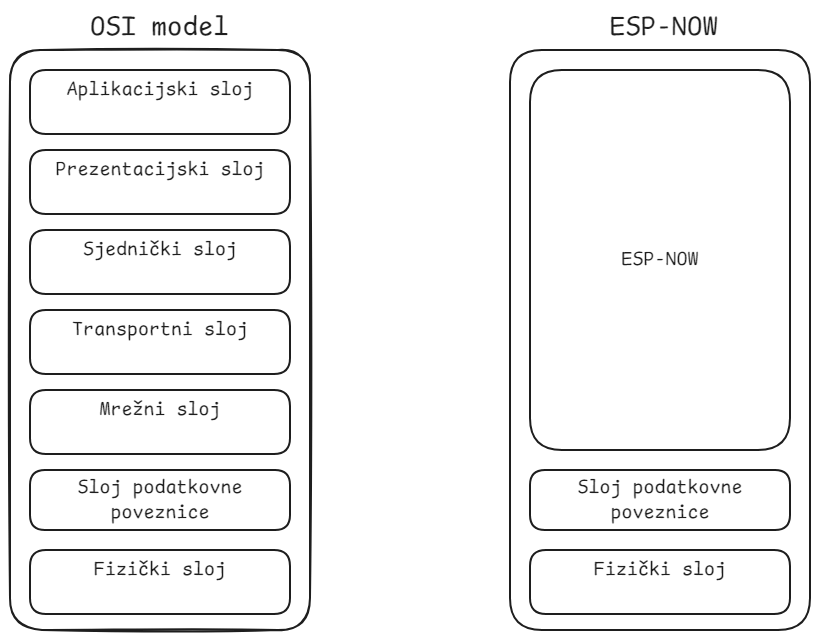
\includegraphics[width=0.8\linewidth]{Figures/osi.png} 
  \caption{Usporedba klasičnog OSI modela s modelom ESP-NOW protkola}
  \label{slk:usporedbaosi}
\end{figure}

Svaki uređaj ima ulogu pošiljatelja i/ili primatelja poruka (obje uloge ako se koristi dvostrani način komunikacije). Uređaji se povezuju s pomoću MAC adresa. 

\section{Načini komunikacije}

Usporedba prikazana na slici (\hyperref[slk:drugaslika]{sl 3.2.})
\\ \\
\textbf{Jedan na jedan} (engl. Unicast One-to-One) \\
Međusobna komunikacija dva uređaja. \\ \\
\textbf{Jedan na više} (engl. Multicast One-to-Many) \\
Jedan uređaj šalje na više uređaja poruku. \\ \\
\textbf{Više na jedan} (engl. Broadcast Many-to-One) \\
Ovaj način podrazumijeva slanje paketa svim uređajima. Mogu ali i ne moraju biti povezani (stavljanjem FF:FF:FF:FF kao MAC adrese poruka se šalje svima).

\begin{figure}[h!]
  \centering
  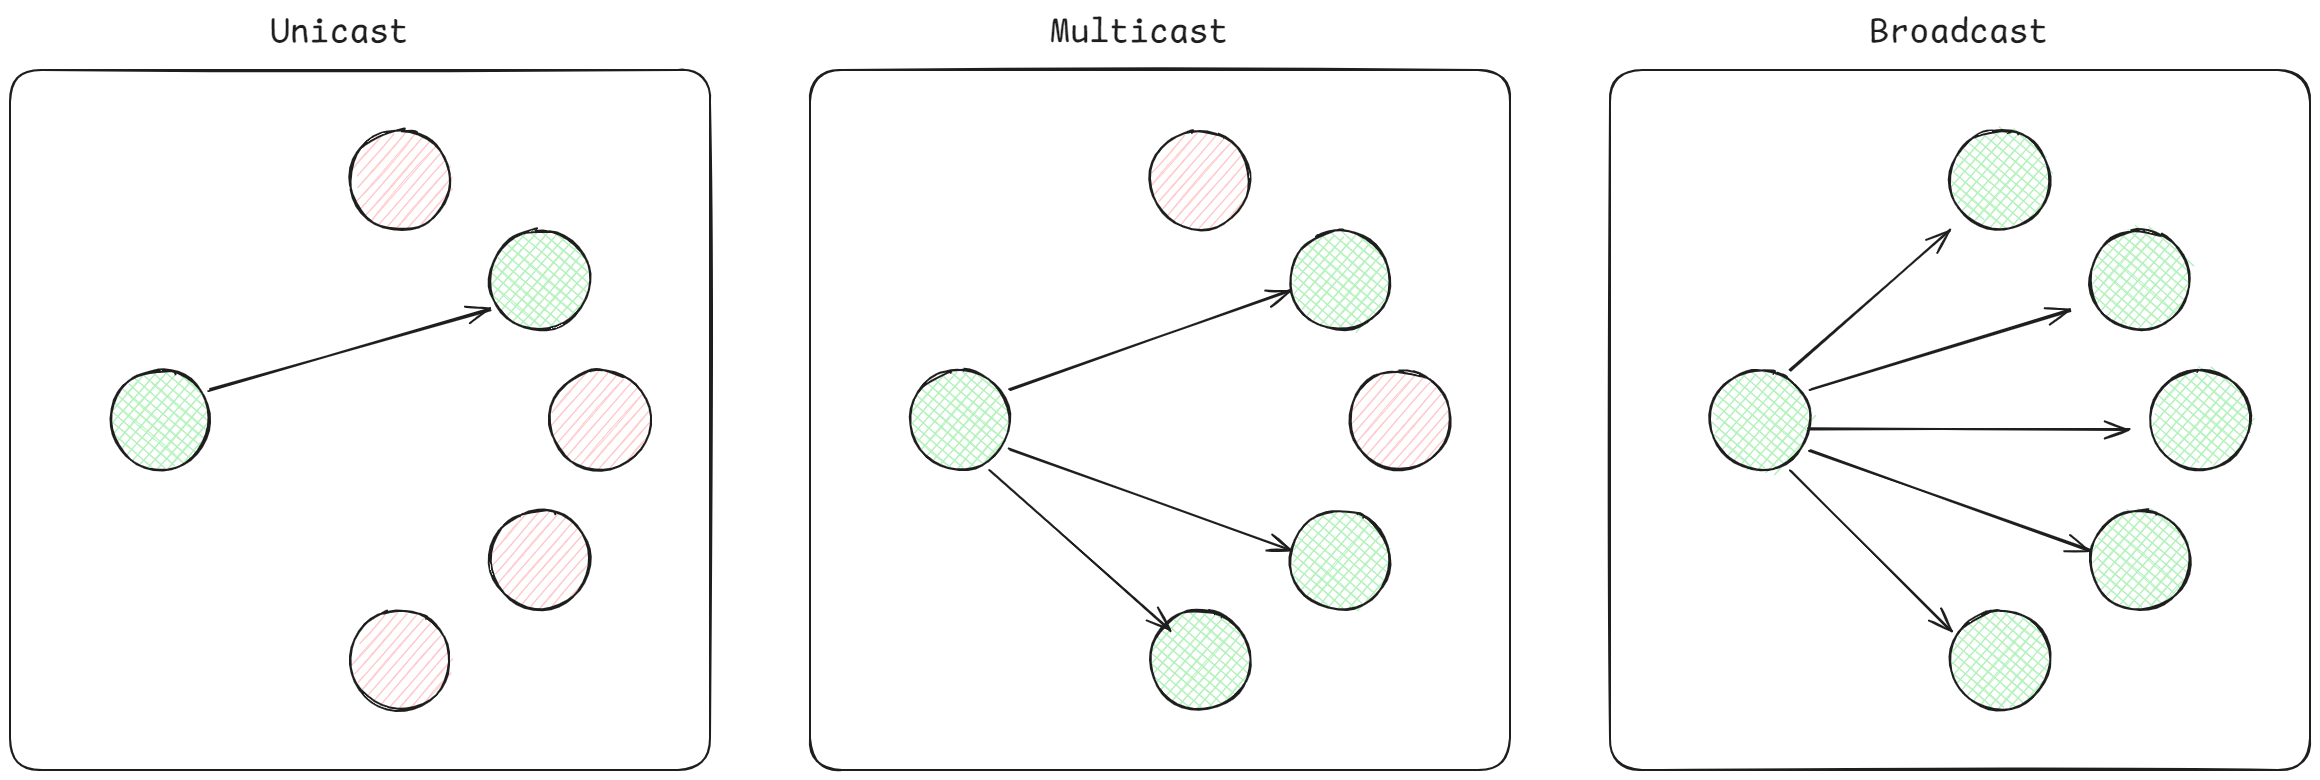
\includegraphics[width=1\linewidth]{Figures/nacini.png} 
  \caption{Usporedba različitih načina komunikacije}
  \label{slk:drugaslika}
\end{figure}

%\section{Struktura paketa}

%Maksimalna veličina paketa je zadana konstantom \verb|ESP_NOW_MAX_DATA_LEN|.

%\begin{table}[h!]
    %\centering
    %\begin{tabular}{|c|c|c|} 
    % \hline
    % \textbf{Polje} & \textbf{Veličina} & \textbf{Opis} \\
    % \hline
    % MAC zaglavlje & 24 bajta & -\\ 
    % \hline
    % Šifra kategorije & 1 bajt & Postavljen na vrijednost 127\\ 
    % \hline
    % Identifikator organizacije & 3 bajta & 0x18fe34 (prva tri bajta MAC adrese)\\ 
    % \hline
    % Nasumična vrijednost & 4 bajta & Služi kao zaštita od napada\\ 
    % \hline
    % Sadržaj & 7-x bajtova & Ovisno o verziji, za 2.0 x = 1532, za 1.0 x = 257\\ 
    % \hline
    % FCS & 4 bajta & Provjera greške\\ 
    % \hline
    %\end{tabular}
    %\caption{Usporedba protokola bežične komunikacije dostupnih na ESP-u}
    %\label{tab:struktura}
%\end{table}

\section{ESP-NOW API}

Detaljnije se može naći na \hyperlink{https://docs.espressif.com/projects/esp-idf/en/v5.4/esp32/api-reference/}{ovom linku}, a u nastavku će biti opisane funkcije koje će se koristiti u kodu.

\subsection{Funkcije inicijalizacije}

Funkcije u ovom dijelu služe za inicijalizaciju potrebnog sklopovlja za komunikaciju.

\verb|esp_err_t nvs_flash_init(void)| \\
Funkcija služi za inicijalizaciju NVS-a (engl. Non-Volatile Storage) koji je potreban za WiFi (spremanje WiFi konfiguracije, ključeva i sl).

\verb|esp_err_t esp_netif_init(void)| \\
Funkcija služi za inicijalizaciju TCP/IP stoga.

\verb|esp_err_t esp_event_loop_create_default(void)| \\
Funkcija napravi petlju događaja koja omogućava drugim komponentama da registriraju \textit{handle}.

\verb|esp_netif_t *esp_netif_create_default_wifi_ap(void)| \\
Funkcija napravi \textit{defaultni} AP (engl. Access Point - \textit{hotspot}).

\verb|esp_err_t esp_wifi_init(const wifi_init_config_t *config)| \\
Inicijalizacija WiFi \textit{drivera} i pokretanje WiFi zadatka. Potrebno je pozvati prije bilo koje druge \verb|wifi| naredbe.

\verb|esp_err_t esp_wifi_set_mode(wifi_mode_t mode)| \\
Postavljenje željenog načina rada (AP, STA ili APSTA).

\verb|esp_err_t esp_wifi_set_config(wifi_interface_t interface, | \\
\verb|wifi_config_t *conf)| \\
Postavljenje željene konfiguracije specificirane u \verb|*conf| varijabli koja je za AP način definirana: 

\begin{verbatim}
typedef struct {
    uint8_t peer_addr[ESP_NOW_ETH_ALEN]; 
    esp_now_role_t role;               
    uint8_t channel;                      
    uint8_t encrypt;                      
    uint8_t lmk[ESP_NOW_KEY_LEN];         
} esp_now_peer_info_t;
\end{verbatim}

\verb|esp_err_t esp_wifi_start(void)| \\
Pokretanje WiFi sučelja s zadanom konfiguracijom.
 
\verb|esp_err_t esp_now_init(void)| \\
Inicijalizira potrebno za ESP-NOW protokol. Potrebno je pokrenuti inicijalizaciju WiFi-ja prije poziva ove funkcije jer ESP-NOW koristi WiFi. 

\verb|esp_err_t esp_now_add_peer(const esp_now_peer_info_t *peer)| \\
Dodaje uređaj za komunikaciju koji je definiran sljedećom strukturom:

\begin{verbatim}
typedef struct {
    uint8_t peer_addr[ESP_NOW_ETH_ALEN]; 
    esp_now_role_t role;               
    uint8_t channel;                      
    uint8_t encrypt;                      
    uint8_t lmk[ESP_NOW_KEY_LEN];         
} esp_now_peer_info_t;
\end{verbatim}

\subsection{Funkcije za web server}

Funkcije u ovom dijelu služe za upravljanje web serverom (prihvaćanje i obrada zahtjeva).

\verb|esp_err_t httpd_start(httpd_handle_t *handle, |\\
\verb|const httpd_config_t *config)| \\
Pokreće web server i alocira memoriju i resurse potrebne za isti kako je zadano u konfiguraciji.

\verb|esp_err_t httpd_register_uri_handler(httpd_handle_t handle, | \\
\verb|const httpd_uri_t *uri_handler)| \\
Registriraj URI handler.

\verb|esp_err_t httpd_req_get_url_query_str(httpd_req_t *r, char *buf, | \\
\verb|size_t buf_len)| \\
Dohvati string iz URL-a

\verb|esp_err_t httpd_query_key_value(const char *query, | \\
\verb|const char *key, char *val, size_t val_size);| \\
Dohvaćanje vrijednosti iz niza oblika: \verb|param1=val1&param2=val2|.

\verb|esp_err_t httpd_resp_send(httpd_req_t *req, const char *buf, | \\
\verb|ssize_t buf_len);| \\
Služi za slanje HTTP odgovora. Podrazumijeva da se cijeli odgovor nalazi u \textit{bufferu}, ako želimo slati u dijelovima koristiti \verb|httpd_resp_send_chunk()|

\verb|esp_err_t httpd_resp_set_type(httpd_req_t *r, const char *type)| \\
Postavlja HTTP content type polje odgovora, podrazumijevana vrijednost je \verb|text/html|.

\subsection{Funkcije za komunikaciju}

Funkcije u ovom dijelu služe za komunikaciju ESP-NOW protokolom.

\verb|esp_err_t esp_now_send(const uint8_t *peer_addr, | \\
\verb|const uint8_t *data, size_t len)| \\
Slanje poruke ESP-NOW protokolom.

\verb|esp_err_t esp_now_register_recv_cb(esp_now_recv_cb_t cb)| \\
Specificiranje callback funkcije (funkcija koja se automatski poziva kada se primi poruka) za primanje ESP-NOW protokolom.

\verb|esp_err_t esp_now_register_send_cb(esp_now_send_cb_t cb)| \\
Isto kao i prethodna samo za slanje poruke.

\section{Sigurnost}

ESP-NOW protokol ima mogućnost slanja enkriptiranih poruka između uređaja. Za enkripciju koristi CCMP metodu uz primarni i lokalni ključ. Primarni ključ se koristi da bi enkriptirao lokalni ključ s AES-128 algoritmom, dok se lokalni koristi za enkripciju poruke CCMP metodom. 

%-------------------------------------------------------------------------------
\chapter{Primjer sustava}
\label{pog:primjer_sustava}

Sustav se sastoji od dva ESP mikroupravljača. Na jednom od njih se vrti web server na koji se možemo spojiti s pomoću računala i on šalje ESP-NOW poruke drugom mikroupravljaču koji prima poruke i obrađuje ih i povremeno šalje poruke prvom upravljaču. Osnovna shema sustava je prikazana na \hyperref[slk:prvaslika]{slici 4.1}

%0x34, 0x86, 0x5D, 0xDC, 0x20, 0xD0
%0x7C, 0x87, 0xCE, 0xF8, 0xC9, 0x59

\begin{figure}[h!]
  \centering
  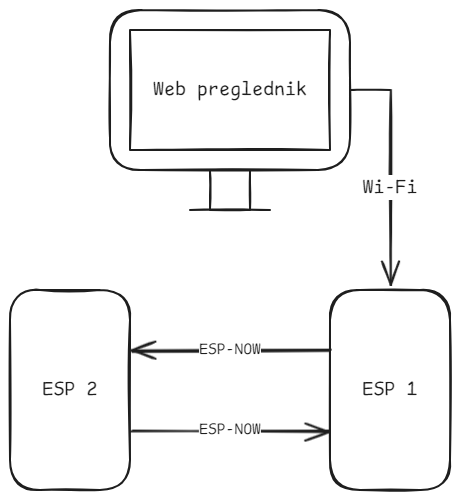
\includegraphics[width=0.6\linewidth]{Figures/sustav.png} 
  \caption{Osnovna shema sustava}
  \label{slk:prvaslika}
\end{figure}

\section{Povezivanje mikrokontrolera i komunikacija s ESP-NOW}
%- drugi prima i salje poruke i mjeri ocitanje temperaturog senzora, kada prodje kritcnu temp treba reagirati odma (sto brze)

Budući da ESP-NOW protokol koristi MAC adresu uređaja za međusobno povezivanje, prvo moramo saznati MAC adresu što možemo napraviti funkcijom \verb|esp_wifi_get_mac|.

Kada znamo MAC adresu možemo uspostaviti ESP-NOW vezu i slati podatke međusobno. Prvo je potrebno inicijalizirati ESP-NOW protokol i registrirati drugi mikrokontroler što je prikazano sljedećim isječkom koda:

\begin{lstlisting}[caption=Inicijalizacija protokola]
nvs_flash_init();

// inicijalizacija WiFi-ja
esp_netif_init();
esp_event_loop_create_default();

wifi_init_config_t cfg = WIFI_INIT_CONFIG_DEFAULT();
esp_wifi_init(&cfg);
esp_wifi_set_mode(WIFI_MODE_APSTA);
esp_wifi_start();

// inicijalizacija ESP-NOW
if (esp_now_init() != ESP_OK) {
    ESP_LOGE(TAG, "ESP-NOW Init Failed");
    return;
}

// registriranje callback funckija za primanje i slanje podataka
esp_now_register_send_cb(on_data_sent);
esp_now_register_recv_cb(on_data_recv);

// spajanje s drugim uredjajem
esp_now_peer_info_t peerInfo = {};
memcpy(peerInfo.peer_addr, sender_mac, 6);
peerInfo.channel = 0;
peerInfo.ifidx = ESP_IF_WIFI_AP; 
peerInfo.encrypt = false;

if (esp_now_add_peer(&peerInfo) != ESP_OK) {
    ESP_LOGE(TAG, "Failed to add peer");
    return;
}

ESP_LOGI(TAG, "ESP-NOW Initialized Successfully");
\end{lstlisting}

Potrebno je inicijalizirati i WiFi sučelje jer ESP-NOW koristi isto. Poruku možemo poslati sljedećim isječkom:

\begin{lstlisting}[caption=Komunikacija ESP-NOW protokolom]
char message[] = "Poruka";
    
esp_err_t result = esp_now_send(receiver_mac, 
    (uint8_t *)message, 
    sizeof(message));

if (result == ESP_OK) {
    ESP_LOGI(TAG, "Message sent successfully");
} else {
    ESP_LOGE(TAG, "ESP-NOW send failed: %s", esp_err_to_name(result));
}
\end{lstlisting}

Primjer komunikacije možemo vidjeti na sljedećem ispisu:

\begin{figure}[h!]
  \centering
  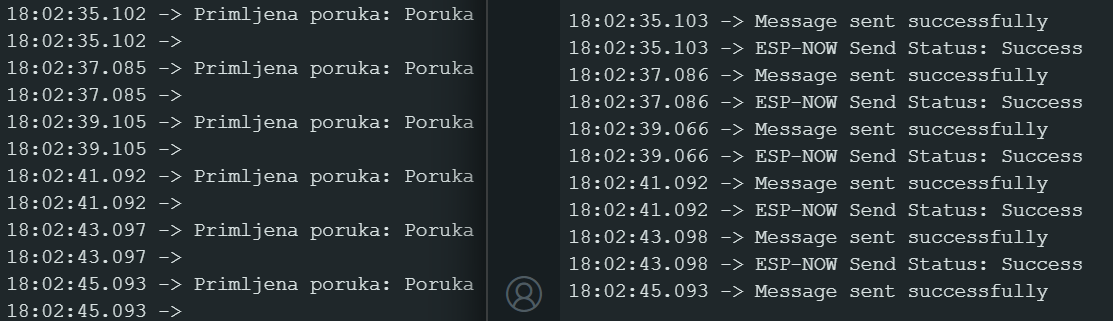
\includegraphics[width=1\linewidth]{Figures/kom.png} 
  \caption{Primjer ispisa ESP-NOW protokolom}
  \label{slk:kom}
\end{figure}

Ako dodatno želimo i mi komunicirati sa sustavom, najpraktičnije bi bilo pomoću nekakvog web sučelja na koji se možemo spojiti pomoću web preglednika. Radi toga, možemo na jednom mikroupravljaču \textit{vrtjeti} i web server na koji se povezujemo. Za to nam je potreban WiFi:

\begin{lstlisting}[caption=Kreiranje WiFi AP-a]
// inicijalizacija WiFi
esp_netif_init();
esp_event_loop_create_default();

esp_netif_t *esp_netif = esp_netif_create_default_wifi_ap();
wifi_init_config_t cfg = WIFI_INIT_CONFIG_DEFAULT();
esp_wifi_init(&cfg);

esp_wifi_set_mode(WIFI_MODE_AP);
wifi_config_t ap_config = {
    .ap = {
        .ssid = "ESP32_AP",
        .ssid_len = strlen("ESP32_AP"),
        .channel = 1,
        .password = "12345678",
        .max_connection = 4,
        .authmode = WIFI_AUTH_WPA_WPA2_PSK
    }
};
esp_wifi_set_config(WIFI_IF_AP, &ap_config);
esp_wifi_start();
\end{lstlisting}

\begin{lstlisting}[caption=\textit{Handler} za http zahtjev]
char query[128];
char message[64] = {0};
    
if (httpd_req_get_url_query_str(req, query, sizeof(query)) == ESP_OK) {
    ESP_LOGI(TAG, "Received Query: %s", query);
    if (httpd_query_key_value(query, "message", message, 
        sizeof(message)) == ESP_OK) {
        ESP_LOGI(TAG, "Extracted Message: %s", message);

        // slanje poruke esp now protokolom
        esp_err_t result = esp_now_send(receiver_mac, 
            (uint8_t *)message, strlen(message));
        if (result == ESP_OK) {
            httpd_resp_send(req, "ESP-NOW Message Sent!", 
                HTTPD_RESP_USE_STRLEN);
            return ESP_OK;
        } else {
            httpd_resp_send(req, "ESP-NOW Message Failed!", 
                HTTPD_RESP_USE_STRLEN);
            return ESP_OK;
        }
    }
}
\end{lstlisting}

Uz pomoć \verb|httpd_req_get_url_query_str| iz zahtjeva izvlačimo parametar koji smo upisali, npr. ako pošaljemo zahtjev \verb|http://192.168.4.1/send?message=hello| (IP \\ adresu ispiše ESP kada je spreman), \verb|httpd_req_get_url_query_str| funkcija će nam vratiti \verb|message=hello|, a potom uz pomoć funkcije \verb|httpd_query_key_value| dobivamo \verb|hello|. \verb|hello|, koji smo pohranili u varijablu \verb|message[]|, šaljemo ESP-NOW protokolom na drugi mikroupravljač.   


%--- ZAKLJUČAK / CONCLUSION ----------------------------------------------------
\chapter{Zaključak}
\label{pog:zakljucak}

TODO


%--- LITERATURA / REFERENCES ---------------------------------------------------

% Literatura se automatski generira / References are automatically generated
% Upiši ime BibTeX datoteke bez .bib nastavka / Enter the name of the BibTeX file without .bib extension
\bibliography{literatura}


%--- PRIVITCI / APPENDIX -------------------------------------------------------

\backmatter

\chapter{Kod}

\begin{lstlisting}[caption=Dohvacanje MAC adrese] 
void print_mac_address() {
    uint8_t mac[6];  // Array to store MAC address

    // Get the MAC address for the WiFi station (WIFI_IF_STA) interface
    esp_err_t ret = esp_wifi_get_mac(WIFI_IF_STA, mac);
    if (ret == ESP_OK) {
        ESP_LOGI(TAG, "ESP32 MAC Address: %02X:%02X:%02X:%02X:%02X:%02X",
                 mac[0], mac[1], mac[2], mac[3], mac[4], mac[5]);
    } else {
        ESP_LOGE(TAG, "Failed to get MAC Address!");
    }
}
\end{lstlisting}

\newpage

\begin{lstlisting}[caption=ESP-NOW sender]
#include <stdio.h>
#include <string.h>
#include "esp_wifi.h"
#include "esp_event.h"
#include "esp_log.h"
#include "esp_now.h"
#include "nvs_flash.h"
#include "esp_netif.h"
#include "esp_http_server.h"

#define TAG "ESP_NOW_SENDER"

uint8_t receiver_mac[] = {0x34, 0x86, 0x5D, 0xDC, 0x20, 0xD0};

/*
 * Callback funkcija za slanje podataka
 * 
 * mac_addr:    MAC adresa uredjaja sa kojeg saljemo podatke
 * status:      status poslane poruke
 * 
 * return:      void
 */
void on_data_sent(const uint8_t *mac_addr, esp_now_send_status_t status) {
    ESP_LOGI(TAG, "ESP-NOW Send Status: %s", 
        (status == ESP_NOW_SEND_SUCCESS) ? "Success" : "Fail");
}

/*
 * Callback funkcija za slanje podataka
 * 
 * recv_info:   podatci o uredjaju sa kojeg smo primili poruku
 * data:        podatci koje primamo
 * len:         velicina polja data
 * 
 * return:      void
 */
void on_data_recv(const esp_now_recv_info_t *recv_info, 
    const uint8_t *data, int len) {
    //const uint8_t *mac_addr = recv_info->src_addr;

    //ESP_LOGI("ESP-NOW", "Received data from: %02X:%02X:%02X:%02X:%02X:%02X",
    //         mac_addr[0], mac_addr[1], mac_addr[2], 
    //         mac_addr[3], mac_addr[4], mac_addr[5]);

    ESP_LOGI("ESP-NOW", "Data: %.*s", len, data);
}

/*
 * Funkcija za inicijalizaciju WiFi-ja u AP nacinu rada kako bi se 
 * mogli povezati preko browsera i slati poruke
 * 
 * return:      void
 */
void init_wifi_ap() {
    esp_netif_init();
    esp_event_loop_create_default();

    esp_netif_t *esp_netif = esp_netif_create_default_wifi_ap();
    wifi_init_config_t cfg = WIFI_INIT_CONFIG_DEFAULT();
    esp_wifi_init(&cfg);

    esp_wifi_set_mode(WIFI_MODE_AP);
    wifi_config_t ap_config = {
        .ap = {
            .ssid = "ESP32_AP",
            .ssid_len = strlen("ESP32_AP"),
            .channel = 1,
            .password = "12345678",
            .max_connection = 4,
            .authmode = WIFI_AUTH_WPA_WPA2_PSK
        }
    };
    esp_wifi_set_config(WIFI_IF_AP, &ap_config);
    esp_wifi_start();

    esp_netif_ip_info_t ip_info;
    esp_netif_get_ip_info(esp_netif, &ip_info);
    ESP_LOGI(TAG, "ESP32 AP IP Address: " IPSTR, IP2STR(&ip_info.ip));
}

/*
 * Funkcija za inicijalizaciju ESPNOW protokola
 * 
 * return:      void
 */
void init_espnow() {
    // inicijalizacija
    if (esp_now_init() != ESP_OK) {
        ESP_LOGE(TAG, "ESP-NOW Init Failed");
        return;
    }

    // registriranje callback funckija za primanje i slanje podataka
    esp_now_register_send_cb(on_data_sent);
    esp_now_register_recv_cb(on_data_recv);

    // spajanje s drugim uredjajem
    esp_now_peer_info_t peerInfo = {};
    memcpy(peerInfo.peer_addr, receiver_mac, 6);
    peerInfo.channel = 0;
    peerInfo.ifidx = ESP_IF_WIFI_AP;
    peerInfo.encrypt = false;

    if (esp_now_add_peer(&peerInfo) != ESP_OK) {
        ESP_LOGE(TAG, "Failed to add peer");
        return;
    }

    ESP_LOGI(TAG, "ESP-NOW Initialized Successfully");
}

esp_err_t get_handler(httpd_req_t *req) {
    char query[128];
    char message[64] = {0};

    if (httpd_req_get_url_query_str(req, query, sizeof(query)) == ESP_OK) {
        ESP_LOGI(TAG, "Received Query: %s", query);
        if (httpd_query_key_value(query, "message", message, 
            sizeof(message)) == ESP_OK) {
            ESP_LOGI(TAG, "Extracted Message: %s", message);

            // slanje poruke esp now protokolom
            esp_err_t result = esp_now_send(receiver_mac, 
                (uint8_t *)message, strlen(message));
            if (result == ESP_OK) {
                httpd_resp_send(req, "ESP-NOW Message Sent!", 
                    HTTPD_RESP_USE_STRLEN);
                return ESP_OK;
            } else {
                httpd_resp_send(req, "ESP-NOW Message Failed!", 
                    HTTPD_RESP_USE_STRLEN);
                return ESP_OK;
            }
        }
    }

    // html stranica
    const char *html_response =
        "<html>"
        "<head><title>ESP32 Sender</title></head>"
        "<body>"
        "<h2>Send a Message via ESP-NOW</h2>"
        "<form action='/send' method='get'>"
        "  <input type='text' name='message' placeholder='Poruka' required>"
        "  <button type='submit'>Send</button>"
        "</form>"
        "</body>"
        "</html>";

    httpd_resp_set_type(req, "text/html");
    httpd_resp_send(req, html_response, HTTPD_RESP_USE_STRLEN);
    return ESP_OK;
}

httpd_handle_t start_server() {
    httpd_config_t config = HTTPD_DEFAULT_CONFIG();
    httpd_handle_t server = NULL;

    if (httpd_start(&server, &config) == ESP_OK) {
        httpd_uri_t uri_get = {
            .uri       = "/send",
            .method    = HTTP_GET,
            .handler   = get_handler,
            .user_ctx  = NULL
        };
        httpd_register_uri_handler(server, &uri_get);
    }
    return server;
}

/*
 * Glavna funkcija iz koje se pozivaju sve potrebne inicijalizacije
 * 
 * return:      void
 */
void app_main() {
    nvs_flash_init();
    init_wifi_ap();
    init_espnow();

    // Message to send
    char message[] = "Hello from ESP-NOW Sender!";
    
    // Send data
    esp_err_t result = esp_now_send(receiver_mac, 
        (uint8_t *)message, 
        sizeof(message));

    if (result == ESP_OK) {
        ESP_LOGI(TAG, "Message sent successfully");
    } else {
        ESP_LOGE(TAG, "ESP-NOW send failed: %s", esp_err_to_name(result));
    }

    start_server();
    ESP_LOGI(TAG, "ESP-NOW Sender with Web Server Ready!");
}
\end{lstlisting}

\newpage

\begin{lstlisting}[caption=ESP-NOW receiver]
#include <stdio.h>
#include <string.h>
#include "esp_now.h"
#include "esp_wifi.h"
#include "esp_event.h"
#include "esp_log.h"
#include "nvs_flash.h"

#define TAG "ESP_NOW_RECEIVER"

uint8_t sender_mac[] = {0x7C, 0x87, 0xCE, 0xF8, 0xC9, 0x59};

/*
 * Callback funkcija za slanje podataka
 * 
 * mac_addr:    MAC adresa uredjaja sa kojeg saljemo podatke
 * status:      status poslane poruke
 * 
 * return:      void
 */
void on_data_sent(const uint8_t *mac_addr, esp_now_send_status_t status) {
    ESP_LOGI(TAG, "ESP-NOW Send Status: %s", 
        (status == ESP_NOW_SEND_SUCCESS) ? "Success" : "Fail");
}

/*
 * Callback funkcija za slanje podataka
 * 
 * recv_info:   podatci o uredjaju sa kojeg smo primili poruku
 * data:        podatci koje primamo
 * len:         velicina polja data
 * 
 * return:      void
 */
void on_data_recv(const esp_now_recv_info_t *recv_info, 
    const uint8_t *data, int len) {
    //const uint8_t *mac_addr = recv_info->src_addr;

    //ESP_LOGI("ESP-NOW", "Received data from: %02X:%02X:%02X:%02X:%02X:%02X",
    //         mac_addr[0], mac_addr[1], mac_addr[2], 
    //         mac_addr[3], mac_addr[4], mac_addr[5]);

    ESP_LOGI("ESP-NOW", "Data: %.*s", len, data);
}

/*
 * Funkcija za inicijalizaciju WiFi-ja
 * 
 * Potrebna jer ESPNOW protokol koristi WiFi pa je potrebno inicijalizirati 
 * hardver zasluzen za WiFi
 * 
 * return:      void
 */
void init_wifi() {
    esp_netif_init();
    esp_event_loop_create_default();

    wifi_init_config_t cfg = WIFI_INIT_CONFIG_DEFAULT();
    esp_wifi_init(&cfg);
    esp_wifi_set_mode(WIFI_MODE_APSTA);
    esp_wifi_start();
}

/*
 * Funkcija za inicijalizaciju ESPNOW protokola
 * 
 * return:      void
 */
void init_espnow() {
    // inicijalizacija
    if (esp_now_init() != ESP_OK) {
        ESP_LOGE(TAG, "ESP-NOW Init Failed");
        return;
    }

    // registriranje callback funckija za primanje i slanje podataka
    esp_now_register_send_cb(on_data_sent);
    esp_now_register_recv_cb(on_data_recv);

    // spajanje s drugim uredjajem
    esp_now_peer_info_t peerInfo = {};
    memcpy(peerInfo.peer_addr, sender_mac, 6);
    peerInfo.channel = 0;
    peerInfo.ifidx = ESP_IF_WIFI_AP; 
    peerInfo.encrypt = false;

    if (esp_now_add_peer(&peerInfo) != ESP_OK) {
        ESP_LOGE(TAG, "Failed to add peer");
        return;
    }

    ESP_LOGI(TAG, "ESP-NOW Initialized Successfully");
}

/*
 * Glavna funkcija iz koje se pozivaju sve potrebne inicijalizacije
 * 
 * return:      void
 */
void app_main() {
    // nvs potreban za WiFi
    nvs_flash_init();
    init_wifi();
    init_espnow();

    // testiranje ESPNOW konekcije
    /* char message[] = "Poruka iz recievera";
    
    esp_err_t result = esp_now_send(receiver_mac, 
        (uint8_t *)message, 
        sizeof(message));

    if (result == ESP_OK) {
        ESP_LOGI(TAG, "Message sent successfully");
    } else {
        ESP_LOGE(TAG, "ESP-NOW send failed: %s", esp_err_to_name(result));
    } */

    ESP_LOGI(TAG, "ESP-NOW Receiver Ready!");
}
\end{lstlisting}
\end{document}
